\chapter{Fundamentos do Desenho de Experimentos}

Neste capítulo você vai aprender sobre a importância do desenho de experimentos e os fundamentos estatísticos desse desenho, com base nos argumentos de \citet{barton_graphical_1999} e \citet{dean_design_1999}, e em aplicações práticas nos campos da educação \citep{schneider_estimating_2007}, gestão \citep{condra_value-added_1995} e indústria \citet{barton_graphical_1999}.

Uma motivação inicial para a aprendizagem pode ser vista em \citet{simple_learning_pro_types_2015}.

O capítulo é complementado por slides na seção a seguir.

\section{Slides}
Ver os slides neste projeto Overleaf, em
4-Computacao-Experimental/aulas/4.2-Estatistica-Experimentacao/slides-desenho-de-experimentos.pdf
%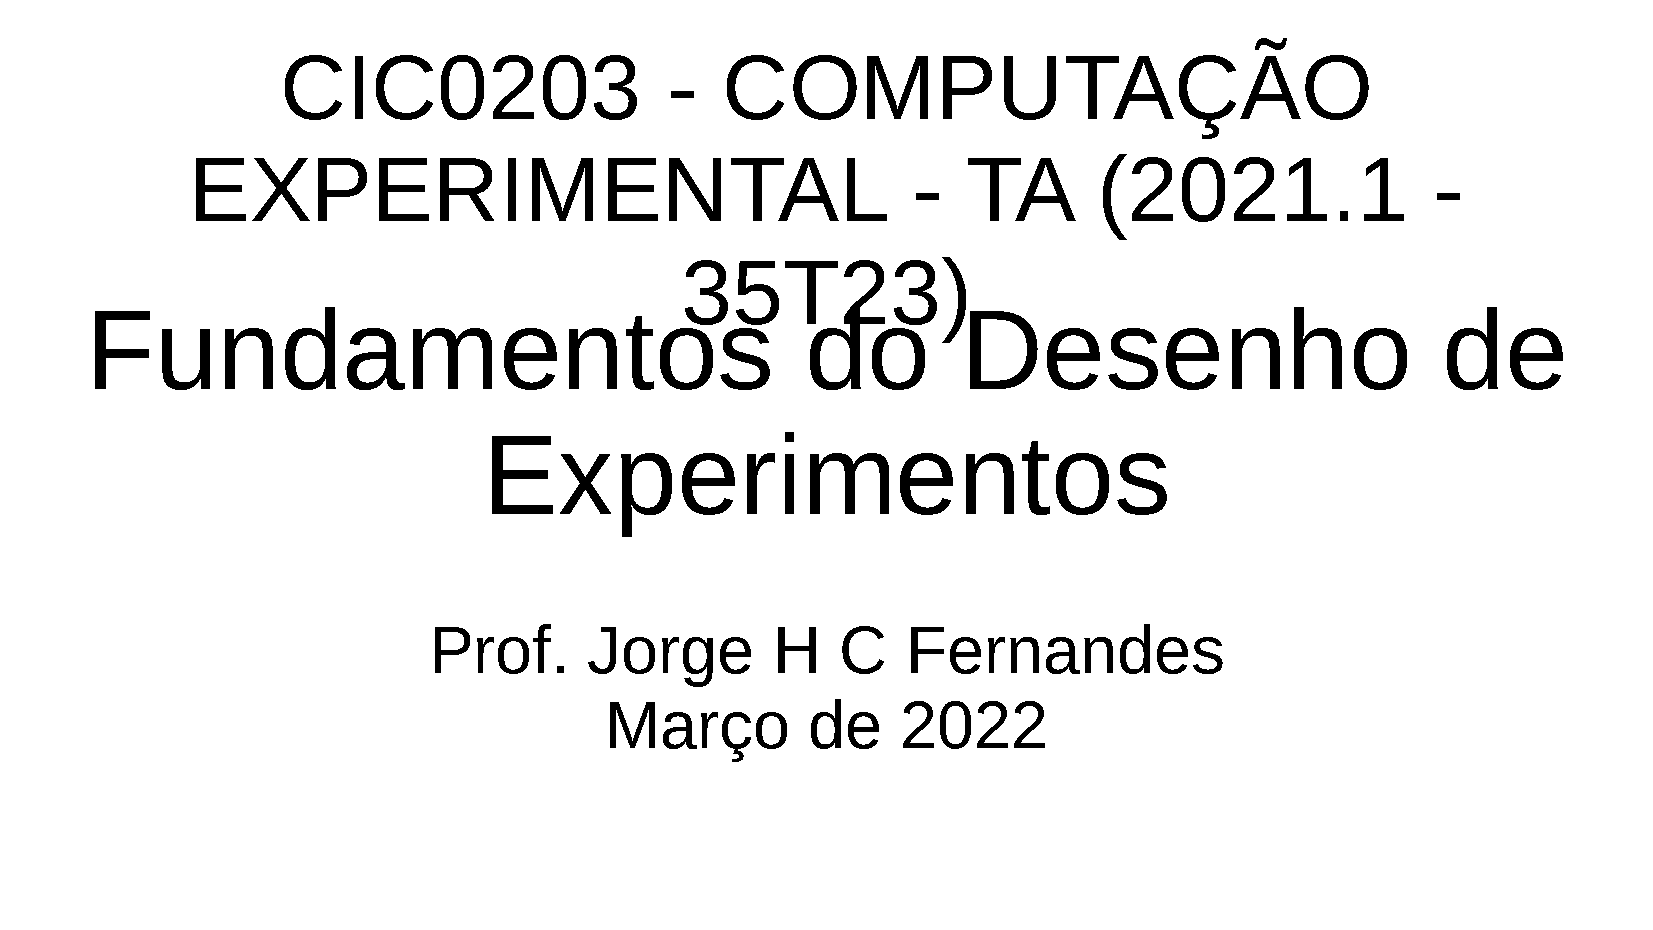
\includepdf[pages=-]{4-Computacao-Experimental/aulas/4.2-Estatistica-Experimentacao/slides-desenho-de-experimentos.pdf}
